\section{Evaluation}
The goal of this evaluation is to investigate the applicability of the proposed matrix-based algorithm to CFPQ with all-path query semantics and to provide a comparison of the most performant linear algebra-based CFPQ algorithms. We will compare the following CFPQ implementations:
\begin{itemize}
	\item $MtxRel$ --- the implementation from~\cite{Azimov:2018:CPQ:3210259.3210264} of the matrix-based CFPQ algorithm for the relational query semantics,
	\item $MtxSingle$ --- the implementation from~\cite{10.1145/3398682.3399163} of the matrix-based CFPQ algorithm for the single-path query semantics,
	\item $MtxAll$ --- the implementation of the proposed matrix-based CFPQ algorithm for all-path query semantics which utilizes SuiteSparse\footnote{SuiteSparse is a sparse matrix software that includes GraphBLAS API implementation. Project web page: \url{http://faculty.cse.tamu.edu/davis/suitesparse.html}. Access date: 20.03.2021.}~\cite{Davis2018Algorithm9S} implementation of GraphBLAS API for matrix manipulations,
	\item $Tns$ --- the implementation from~\cite{kron} of the Kronecker product-based CFPQ algorithm for all three query semantics including the all-path query semantics.
	
\end{itemize}

	

%{\setlength{\tabcolsep}{0.25em}
%	\begin{table*}[t]
%		{
%			\caption{Index creation time in seconds and memory in megabytes where we use "$err$" in case of out of memory error }
%			\label{tbl:index_creation}
%			\small
%			\rowcolors{4}{black!2}{black!10}
%			\begin{tabular}{|l|l|l|l|l|l|l|l|l|l|l|l|l|l|l|l|l|l|l|}
%				\hline
%				\multicolumn{1}{|c|}{\multirow{3}{*}{Graph}} & \multicolumn{1}{c|}{\multirow{3}{*}{\#V}} & \multicolumn{1}{c|}{\multirow{3}{*}{\#E}} & \multicolumn{8}{c|}{G1}                                                                                               & \multicolumn{8}{c|}{G2}                                                                                               \\ \cline{4-19} 
%				\multicolumn{1}{|c|}{}                       & \multicolumn{1}{c|}{}                     & \multicolumn{1}{c|}{}                     & \multicolumn{2}{c|}{MtxRel} & \multicolumn{2}{c|}{MtxSingle} & \multicolumn{2}{c|}{MtxAll} & \multicolumn{2}{c|}{Tns} & \multicolumn{2}{c|}{MtxRel} & \multicolumn{2}{c|}{MtxSingle} & \multicolumn{2}{c|}{MtxAll} & \multicolumn{2}{c|}{Tns} \\ \cline{4-19} 
%				\multicolumn{1}{|c|}{}                       & \multicolumn{1}{c|}{}                     & \multicolumn{1}{c|}{}                     & Time         & Mem          & Time        & Mem        & Time           & Mem           & Time         & Mem          & Time         & Mem          & Time        & Mem        & Time           & Mem           & Time         & Mem          \\ \hline
%				pathways                                     & 6 238                                     & 18 598 & 0.01         & 140 & 0.01           & 671                                     & 0.04         & 91           & 0.02        & 123                             & 0.01         & 140  & 0.01           & 671 & 0.01         & 49           & 0.01        & 122               \\ \hline
%				go-hierarchy                                 & 45 007                                    & 980 218                                   & 0.08         & 254  & 1.41           & 660 & 22.12        & 38797        & 0.17        & 265                            & 0.09         & 255 & 0.84           & 671 & 0.35        & 195        & 0.24        & 252                             \\ \hline
%				enzyme                                       & 48 815                                    & 109 695                                   & 0.01         & 181 & 0.01           & 216 & 0.4          & 307          & 0.04        & 137                              & 0.01         & 181 & 0.01           & 217 & 0.02         & 61           & 0.02        & 132                            \\ \hline
%				eclass\_514en                                & 239 111                                   & 523 727                                   & 0.07         & 180  & 0.23           & 216 & 25.02        & 14416        & 0.24        & 205                            & 0.06         & 181 & 0.16           & 216    & 0.22         & 126          & 0.27        & 193                         \\ \hline
%				go                                           & 272 770                                   & 534 311                                   & 1.00         & 244  & 1.45           & 215 & 11.8         & 8290         & 1.58        & 282                          & 0.94         & 246  & 0.93           & 217  & 1.13         & 990          & 1.27        & 243                          \\ \hline
%				geospecies                                   & 450 609                                   & 2 311 461                   & 0.02         & 212    & 0.06           & 2250           & 4.45         & 2691         & 0.08        & 218                          & 0.01         & 248 & 0.01           & 2251            & 0.34         & 156          & 0.01        & 196              \\ \hline
%				taxonomy                                     & 5 728 398                                 & 14 922 125                             & 1.13         & 965     & 2.73           & 1962               & $err$        & $err$        & 4.42        & 2018       & 0.72         & 1175      & 1.15           & 2250    & 3.84        & 1507        & 3.56        & 1776                   \\ \hline
%			\end{tabular}
%		}
%	\end{table*}
%}


%{\setlength{\tabcolsep}{0.25em}
%	\begin{table}
%		{
%			\caption{Index creation time in seconds and memory in megabytes for $geo$ query}
%			\label{tbl:index_creation_geo}
%			\small
%			\rowcolors{4}{black!2}{black!10}
%				\begin{tabular}{|c|l|l|l|l|l|l|l|l|}
%					\hline
%					\multirow{2}{*}{Graph}           & \multicolumn{2}{c|}{MtxRel} & \multicolumn{2}{c|}{MtxSingle} & \multicolumn{2}{c|}{MtxAll} & \multicolumn{2}{c|}{Tns} \\ \cline{2-9} 
%					& Time         & Mem          & Time        & Mem        & Time           & Mem           & Time         & Mem          \\ \hline
%					\multicolumn{1}{|l|}{geospecies} & 7.48         & 7645     & 15.54          & 22941 & 32.06        & 44235        & 26.32       & 19537                   \\ \hline
%				\end{tabular}
%		}
%	\end{table}
%}


All implementations utilize CPU and use matrices in sparse format (CSR). First, we measured the execution time and required memory of the index creation. Then we compared the practical applicability of the paths extraction for both implementations $MtxAll$ and $Tns$ of the CFPQ with all-path query semantics. The source code is available on GitHub\footnote{Sources of all CFPQ implementations: \url{https://github.com/JetBrains-Research/CFPQ\_PyAlgo}. Access date: 20.03.2021.}.

For evaluation, we used a PC with Ubuntu 18.04 installed.
It has Intel core i7-6700 CPU, 3.4GHz, and DDR4 64Gb RAM.
We only measure the execution time of the algorithms themselves, thus we assume an input graph is loaded into RAM in the form of its adjacency matrix in the sparse format.

\subsection{Dataset Description}

We use the graphs and respective queries from the CFPQ\_Data dataset\footnote{CFPQ\_Data dataset GitHub repository: \url{https://github.com/JetBrains-Research/CFPQ_Data}. Access date: 20.03.2021.} provided in~\cite{10.1145/3398682.3399163} that contains the real-world RDFs, query $geo$ for the $geospecies$ graph, and query $g2$ for other graphs. These queries are variations of the \textit{same-generation query}~\cite{FndDB} --- an important example of real-world queries that are context-free but not regular.




\subsection{Evaluation Results}
%\begin{figure*}
%	\begin{subfigure}{0.32\textwidth}
%		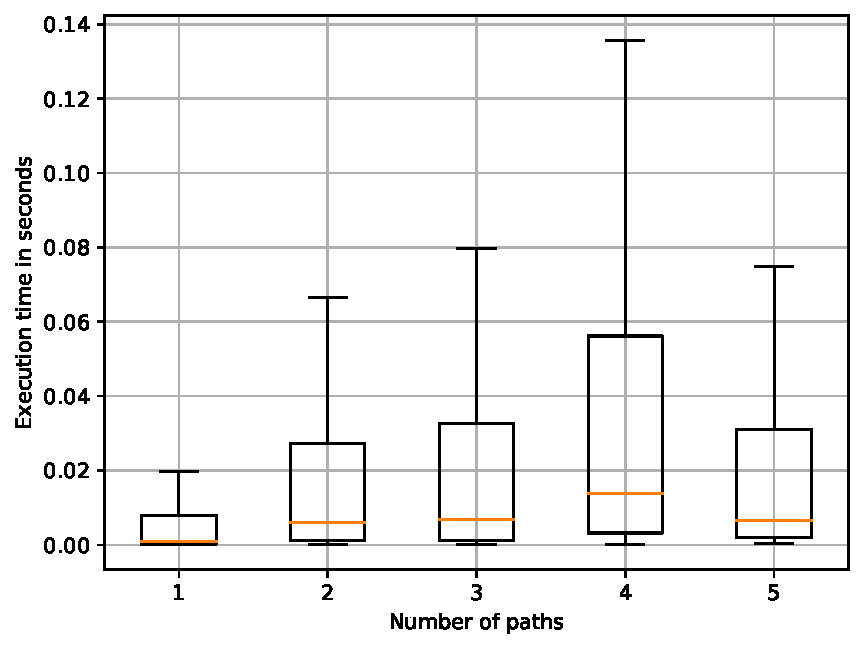
\includegraphics[width=\linewidth,trim=0 0 -1.5cm 0]{pictures/tensor_go_10_small.pdf}
%		\caption{small number of paths} \label{fig:extractTimeGoSmallTns}
%	\end{subfigure}
%	\hspace*{\fill} % separation between the subfigures
%	\begin{subfigure}{0.32\textwidth}
%		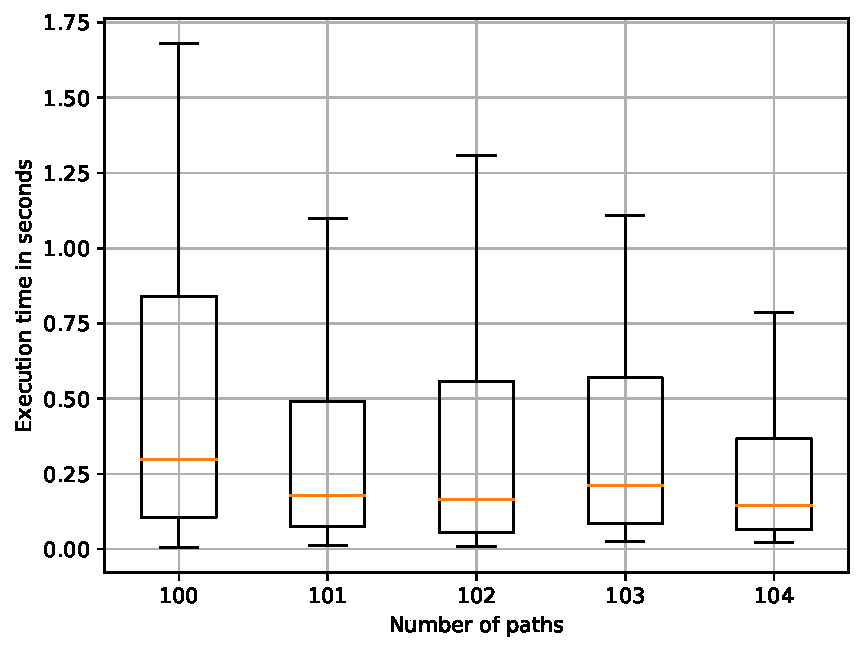
\includegraphics[width=\linewidth,trim=0 0 -1.5cm 0]{pictures/tensor_go_10_big.pdf}
%		\caption{medium number of paths} \label{fig:extractTimeGoMedTns}
%	\end{subfigure}
%	\hspace*{\fill} % separation between the subfigures
%	\begin{subfigure}{0.32\textwidth}
%		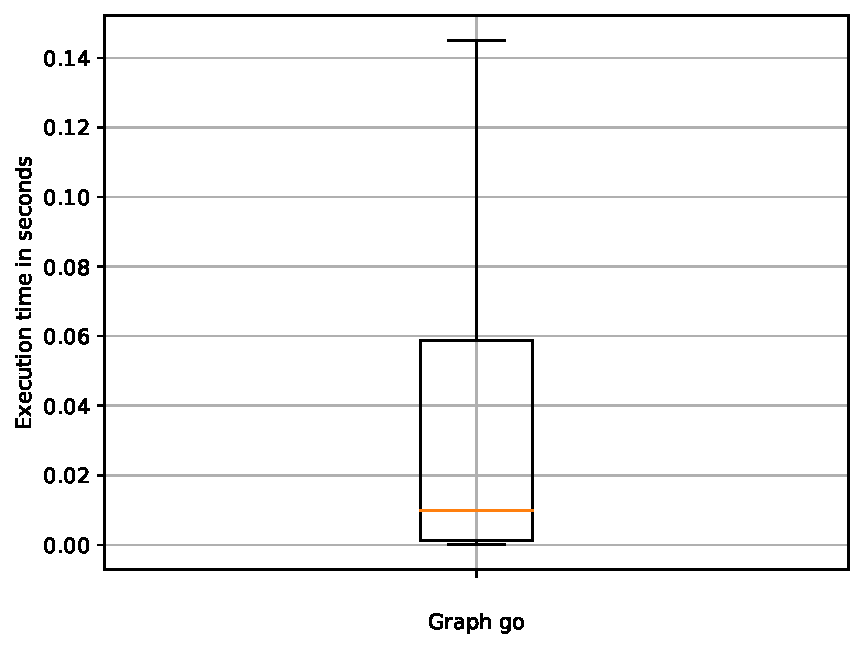
\includegraphics[width=\linewidth,trim=0 0 -1.5cm 0]{pictures/go_10_all_tensor.pdf}
%		\caption{average path extraction time} \label{fig:extractTimeGoAverageTns}
%	\end{subfigure}
%	\caption{Execution time of the Kronecker product-based path extraction algorithm from~\cite{kron} implemented in $Tns$ for the graph $go$}
%	\label{fig:extractTimeTns}
%\end{figure*}

\begin{figure*}
	\begin{subfigure}{0.32\textwidth}
		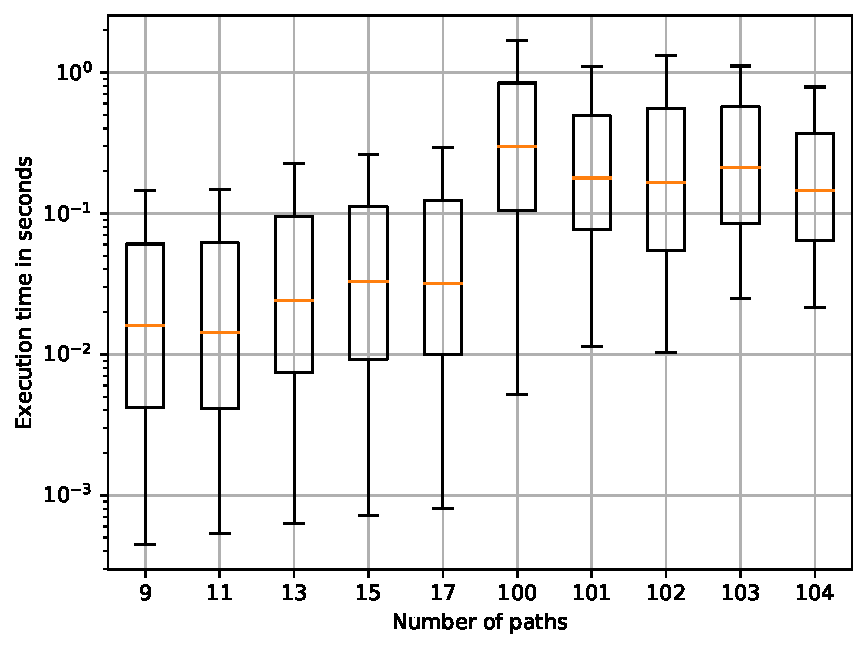
\includegraphics[width=\linewidth,trim=0 0 -1.5cm 0]{pictures/tensor_go_10_big_small.pdf}
		\caption{$Tns$ path extraction depending on number of paths} \label{fig:extractTimeGoMtx}
	\end{subfigure}
	\hspace*{\fill}
	\begin{subfigure}{0.32\textwidth}
		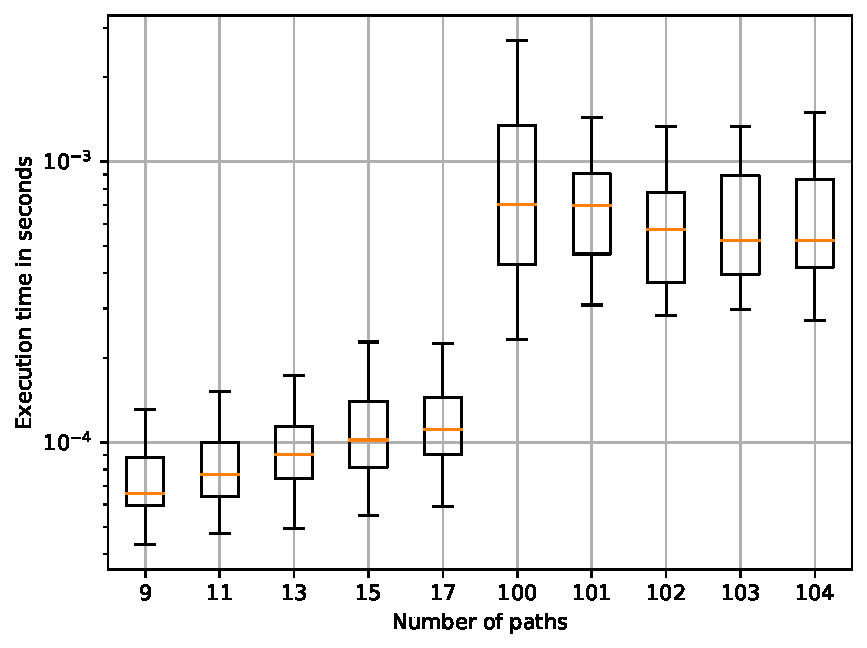
\includegraphics[width=\linewidth,trim=0 0 -1.5cm 0]{pictures/allMatr_go_10_big_small.pdf}
		\caption{$MtxAll$ path extraction depending on number of paths} \label{fig:extractTimeGoTns}
	\end{subfigure}
	\hspace*{\fill} % separation between the subfigures
	\begin{subfigure}{0.32\textwidth}
		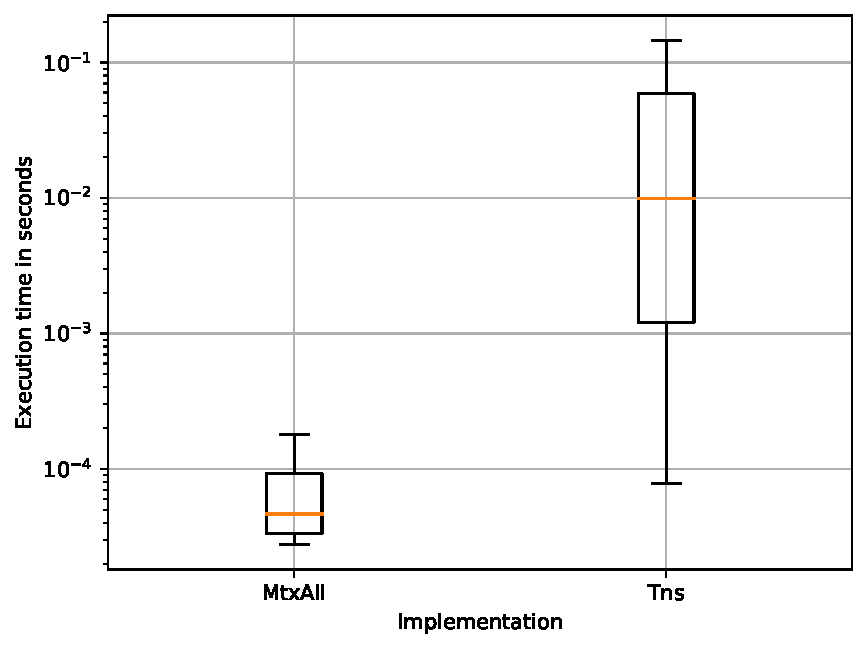
\includegraphics[width=\linewidth,trim=0 0 -1.5cm 0]{pictures/go_10_all_matrixall_tensor.pdf}
		\caption{average path extraction time} \label{fig:extractTimeGoAverage}
	\end{subfigure}
	
	\caption{Execution time of the proposed matrix-based path extraction algorithm implemented in $MtxAll$ and the Kronecker product-based path extraction algorithm from~\cite{kron} implemented in $Tns$ for the graph $go$}
	\label{fig:extractTime}
\end{figure*}

The results of the index creation for all implementations are presented in Table~\ref{tbl:index_creation}. We can see that the most performant index creation is in $MtxRel$ implementation, especially on big graphs. But $MtxRel$ is applicable only for relational query semantics  and cannot restore any paths of interest. Thus, for relational query semantics we can use a more simple index (Boolean matrices) to only solve the reachability problem. The $MtxSingle$ implementation constructs the index up to 2 times slower on big graphs and consumes more memory. This is the cost of storing additional information in the index for the single-path query semantics to be able to restore only one path for each vertex pair. The $MtxAll$ and $Tns$ implementations construct the index up to 2-3 times slower than the $MtxSingle$ implementation and also consumes even more memory, especially on big graphs like $geospecies$ with complex structure for the same-generation query. These two implementations support the all-path query semantics and make it possible to restore all paths corresponding to the same-generation query. However, the Kronecker product-based implementation $Tns$ uses a more complex but compact index and consumes less memory. The implementation $MtxAll$ of the proposed matrix-based CFPQ algorithm for all-path query semantics has comparable execution time to $Tns$  on small graphs but $MtxAll$ is significantly slower and consumes more memory on some big graphs with complex structure than $Tns$. The reason for such behavior is that the proposed matrix-based algorithm is trying to store the information of all founded paths more explicitly, and the index constructed by $MtxAll$ is less compact than the one constructed by $Tns$.

After constructing the index, we compared the execution time of the path extraction for CFPQ with all-path query semantics using both $MtxAll$ and $Tns$ implementations. The results of path extraction for graph $go$ are presented in Figure~\ref{fig:extractTime} (boxplots are standard, medians are indicated and outliers are omitted). For computation termination, we limit the maximum path length to 10 since most of the paths of interest in the graph $go$ satisfy this constraint. After that, we extract paths for each vertex pair and group the execution time by the number of paths returned in Figures~\ref{fig:extractTimeGoMtx} and \ref{fig:extractTimeGoTns} (not all number of paths are presented). Also, we provide the average path extraction time for both implementations and graph $go$ in Figure~\ref{fig:extractTimeGoAverage}. Note that the global medians in Figure~\ref{fig:extractTimeGoAverage} are lower than all the respective medians shown in the Figures~\ref{fig:extractTimeGoMtx} and \ref{fig:extractTimeGoTns} since there are many vertex pairs in the graph $go$ with the number of found paths less than 9. We can see that the path extraction running time of the implementation $MtxAll$ of the proposed matrix-based algorithm is up to 1000 times faster than for the Kronecker product-based implementation $Tns$. As was mentioned above, in the proposed matrix-based CFPQ algorithm we construct an index with more explicit information about all paths found. Thus, paths can be restored significantly faster than using the Kronecker product-based algorithm.

We can conclude the following.
\begin{itemize}
	\item Our evaluation allows us to conclude that the most performant linear algebra-based algorithm for the CFPQ with relational and single-path query semantics are matrix-based algorithms from~\cite{Azimov:2018:CPQ:3210259.3210264} and \cite{10.1145/3398682.3399163} respectively.
	\item For all-path query semantics, the proposed matrix-based and the Kronecker product-based CFPQ algorithms have the following tradeoffs. If it is necessary to frequently recalculate the index for a changing graph or a path query then the best choice is the Kronecker product-based algorithm~\cite{kron} with faster and less memory consuming index construction. If it is necessary to extract paths many times for a once constructed index or index changes can be efficiently computed dynamically then the proposed matrix-based CFPQ algorithm is preferable.
\end{itemize}



